%
%  アブストラクトのサンプルファイル (UTF-8)
%
%   Updated: 2016/12/01 Kou Fujimoto (kou-f@mail.dendai.ac.jp)
%   prepared by Takayuki Okuno (t_okuno@ms.kagu.tus.ac.jp)
%
\documentclass[twoside,twocolumn,10pt]{jarticle}  % 2段組の場合
%\documentclass[11pt]{jarticle}   % 1段組の場合
\usepackage{latexsym,amssymb}
%\usepackage[dvips]{graphicx} % epsファイルを使う場合
\usepackage[dvipdfmx]{graphicx}
\usepackage{orsabs-utf8}
\usepackage{amsmath}
% \usepackage{nccmath}
\usepackage{algorithm}
\usepackage{enumerate}
\usepackage[hyphens]{url}
\newcommand{\bm}[1]{{\mbox{\boldmath $#1$}}}
%%%%%%%%%% Title %%%%%%%%%%%%%%%%%%%%%%%%%%%%%%%%%
\title{OpenPNEのソフトウェアエージングに関する研究}
\author{\begin{tabular}{lll@{}ll}
         & 東京都立大学 & *&近藤和希 & KONDO Kazuki \\
        会員 & 東京都立大学 &  &肖霄 & XIAO Xiao
        \end{tabular}}
\date{}
\begin{document}
\maketitle
%%%%%%%%%% ここから本文%%%%%%%%%%%%%%%%%%%%%%%%%%%
\section{序論}
現代では,ソフトウェアは私たちの身の回りから宇宙規模のシステムに至るまで,非常に長時間の連続稼働が必要なものが多く存在する.
そのような連続稼働によって予期しない性能劣化が生じる現象は「ソフトウェアエージング」と呼ばれ,特に高可用性が要求されるソフトウェアにおいては,ソフトウェアエージングのリスクを定量的に評価する必要性が高まっている.
% 特に,ソフトウェアエージング関連の障害は,開発の段階で発見し,完全に原因を解決することは難しいものであるとも述べられている\cite{Grottke2007Fightinga}.\par
% 1990年代初頭から,ソフトウェアエージングに関する広範な研究が行われてきた.
% しかし,ソフトウェアエージングの振舞はソフトウェアシステムの種類によって異なる.
% そのため,ソフトウェアエージングのリスクを評価することは,ソフトウェアシステムの種類ごとに不可欠だと言える.
% 身近なデジタルサービスから社会的な機能を提供する現代のソフトウェアシステムの多くは,伝統的なクライアント/サーバーシステムで構築され様々な種類が存在する.
% いくつかの研究\cite{Grottke2006Analysis}\cite{Alonso2010Adaptive}\cite{Alonso2011Predicting}\cite{Magalhaes2010Prediction}は,これらのシステムを評価している.\par
% また,ソフトウェアエージングのリスクが観測された場合,次に検討すべきはソフトウェア若化手法の検討である.
% ソフトウェアエージング関連のバグが蓄積し,それがシステムの性能劣化として現れることを未然に防ぐことが目的である.

本研究では,ソフトウェアエージングの研究対象として,SNSシステムの一つであるOpenPNE\footnote{https://www.openpne.jp/about/}を選択する.
% SNSならではの変動する負荷期間を想定し,共通の監視期間における三種類のメトリクスに着目し,ソフトウェアエージングのリスク調査を目指す.
動機付けは,X\footnote{https://about.x.com/ja}のようなSNSシステムは,高い拡張性を持ち,膨大なユーザー数を抱えており,企業にとってサーバー運用のリスクが高まっているためである.
また,これまでのソフトウェアエージングに関する研究の中で,SNSシステムを対象にしたものは,調査の限りない.
本研究では,Measurement-based Approach\cite{Dohi2020Handbook}に基づき,SNSシステムの特徴を踏まえた負荷シナリオを設定し,各シナリオに対して,負荷期間と監視期間\cite{Torquato2018SWAREa}を設けることで,SNSシステムにおけるソフトウェアエージングのリスクを調査する.
% \section{研究目的}
% \subsection{関連研究}
% 1984年にAdams\cite{Adams1984Optimizing}による継続的なソフトウェア稼働によるパフォーマンスの低下が報告された後,1994年にParnas\cite{Parnas1994Software}によってソフトウェアエージングという用語が最初に使用されたとき,多くの研究者は驚かされ,それ以来広範な研究が行われてきた.
% 複数のソフトウェアエージングの定義が存在するが,本研究では,Huangら\cite{Huang1995Software}によるシステムの実行時間に焦点を当てたプロセスエージングと呼ばれるソフトウェアエージングの定義に基づき考える.
% % Parnas\cite{Parnas1994Software}は,ソフトウェアエージングを次のように定義している.
% % 「ソフトウェアエージングには,2つの,非常に異なるタイプがある.
% % 1つ目は,製品の所有者が変化するニーズに合わせて製品を変更できなかったことが原因である.
% % 2つ目は,行われた変更の結果である.」
% % 1年後の1995年,Huangら\cite{Huang1995Software}は,プロセスエージングと呼ばれる,広く受け入れられているソフトウェアエージングの定義を提供した.
% % 「プロセスのエージングは,数日から数週間の実行でアプリケーションプロセスが劣化することに関連している」.
% % これらの定義の主な違いは,前者がソフトウェアの保守の側面を包含しているのに対し,後者は実行時間に焦点を当てていることである.

% Dohiら\cite{Dohi2020Handbook}によると,ソフトウェアエージングの研究は,Threshold-based Approach,Machine learning-based Approach,Measurement-based Approachの3つの手法に分類できる.
% 本研究では特に,Measurement-based Approachを用いた研究について調査し,多種多様なシステムを対象に行われていることが分かった.
% 以下,書き方1と2のどちらかで検討中.
% 1.例として,IBMのクラウドシステム\cite{Sukhwani2017Monitoringa}や画像判定アプリケーションをクラウド環境やエッジ環境にデプロイしたもの\cite{Andrade2020Softwarea}\cite{Andrade2021Memorya}\cite{Andrade2023Comparativea},さらにAndroid OS\cite{Araujo2013Investigative}\cite{Cotroneo2016Software}\cite{Cotroneo2020Comprehensive}やブロックチェーンにまで至る.
% 2.本分野の研究は,Webアプリケーション\cite{Grottke2006Analysis}\cite{Matias2006Experimental}やクラウドシステム\cite{Sukhwani2017Monitoringa}\cite{Andrade2020Softwarea}\cite{Andrade2021Memorya}\cite{Andrade2023Comparativea}といった多種多様なシステムを対象にし,それぞれのソフトウェアエージングの振舞とその原因を調査している.
% % Threshold-based Approachでは,指定された閾値を超える時間を予測する研究や,平均応答時間\cite{Silva2007Using},仮想メモリ使用量\cite{Matias2006Experimental},メモリ使用量\cite{Araujo2011Software}\cite{Avritzer2006Performance}を評価指標として閾値を決定する方法を提案する研究が行われてきた.
% % Threshold-based Approachだけでは,ソフトウェアシステムを活性化し若化を行うために最適な時期を見つけるには不十分だが,他の2つのアプローチと組み合わせて使用される.

% % Machine learning-based Approachでは,上記の2つのアプローチに機械学習を適用して,精度を高めている\cite{Alonso2010Adaptive}.
% % 機械学習の分類を使用して,ソフトウェアエージングによって引き起こされる異常を特定する試みがいくつか行われている\cite{Alonso2011Predicting}.
% % Measurement-based Approachでは,Mann-Kendall検定とSenの傾き推定を使用したソフトウェアの経年劣化の検出\cite{Garg1998Methodologya},主成分分析\cite{Cotroneo2010Software}を使用したソフトウェアエージングの識別,ログデータを使用した因子分析など,ソフトウェアエージングの定量化に多くの労力が注がれてきた.
% % さらに,いくつかの論文では,ソフトウェアエージングによるリソースの枯渇時間を推定し,エージングに関連する障害を予測している\cite{Chen2018ARFPredictor}.
% % 測定するメトリクスの中でも特に,メモリについては「メモリの枯渇に焦点を当てるのは,メモリのTTE(Time To Exhaustion)がコンピュータシステムのリソースの中で最も低く,メモリ管理のバグ(メモリリークなど)が最も顕著なソフトウェアエージングの原因である」と述べられている\cite{Cotroneo2010Softwarea}.
% % 以下では,この手法を用いた研究を,対象となるシステムや環境ごとに分類し紹介する.
% % クラウド
% % まず初めにクラウドシステムに関するものを挙げる.
% % Sukhwaniら\cite{Sukhwani2017Monitoringa}は,2017年にIBM独自のクラウドシステムのソフトウェアエージング現象の調査を行い,リソースの枯渇予測やそれを利用した警告システムの搭載を実現した.
% % この研究では,彼らは閾値の検討にも取り組んでいる.
% % Andradeら\cite{Andrade2020Softwarea}は,2020年に画像判定アプリケーションをクラウド環境とエッジ環境上でそれぞれ長時間運用し,メモリやCPUのリソースを監視し,エージングの動向を比較した.
% % さらに2021年には.同じアプリケーションを,パブリッククラウド環境とプライベートクラウド環境で運用し,使用可能メモリの観点から,それぞれのエージングの潜在可能性を指摘した\cite{Andrade2021Memorya}.
% % しかし,前者はGoogleデーモンプロセスに,後者はファイルのインデックス作成プロセスというように,それぞれ異なる原因として関連付けた.
% % さらに,2023年には2020年の研究の延長として,ユーザー感知メトリクスとして,画像判定アプリケーションの応答時間ではなく,スループット損失に着目した\cite{Andrade2023Comparativea}.
% % そこでは,プロセスレベルでの原因分析に取り組むため,メモリ消費量の多い上位6つのプロセスとRSS(Resident Set Size)の相関関係および因果関係の調査を行った.
% % なお,因果関係の調査には,時系列データセットの移動エントロピーを分析している.
% % % Android OSとブロックチェーン
% % Araujo\cite{Araujo2013Investigative}らは,2013年にAndroid OSのソフトウェアエージングを調査するための方法論を提案し,継続的なリソース監視により,メモリリークの検出に成功している.
% % さらに,Cotroneo\cite{Cotroneo2016Software}らは2016年に,起動時間LTの遅延現象を,ユーザー感知メトリクスおよびリソースメトリクスの監視を行い相関を調べた.
% % その後,彼らは2020年に原因特定のため,ガベージコレクションの遅延現象を探り,javaコンテナのメモリフラッシュによるリジュベネーションの成功にまで研究を広げた\cite{Cotroneo2020Comprehensive}.
% % また,peer-to-peerシステムであるブロックチェーンシステムを扱うものもある.添田さんの論文を参考文献に.
% \subsection{動機}
% OpenPNEとは,株式会社手嶋屋が中心となって,OSS方式で開発されてきたSNS構築ソフトウェアである\footnote{https://www.openpne.jp/about/}.
% 開発の敷居が比較的低く,NHK出版やガンホーゲームのファンサイトなど複数の導入事例もあるSNSということで選択した.
% SNSならではの拡張性の高さも備えており,セットアップに関して,多数の文書が提供されていることも後押しになった.
% また,SNSシステム独自のアクセス負荷の時系列変化も考えられる\footnote{https://note.fuller-inc.com/n/ne35c0cdba519}.
% そして,機能も非常に複雑で高層的な処理が必要になるため,サーバーのメトリクス(CPUやメモリ)に代表されるようなSNSに関するあらゆるメトリクスを分析し評価する必要性があると考えられる.
% そのため,現実のユーザーの運用とは異なると述べられている論文もある\cite{Andrade2023Comparativea}.
% 負荷シナリオの検討においては,なるべくシンプルでありながら,ソフトウェアエージングを引き出すようなバランスの取れたストレステストの考案が必要であると考えられる\cite{Cotroneo2016Software}.
% また,本研究では,Torquatoら\cite{Torquato2018SWAREa}が2018年に,ストレス期間,待期期間,若化期間のそれぞれでリソースの監視を行った研究を参考にし,本研究では監視期間というものを考える.
% ただし,本研究では若化期間には踏み込まない.

\section{実験環境}\label{sec:environment}

図\ref{fig:1}に示す実験環境は2台のデバイスで構成されている.
サーバーPCでは,Dockerを用いてWindows OSとOpenPNEの運用環境を隔離している.
この設定によりOpenPNE環境を独立させ,移植性が向上し,クリーンなメトリクスの取得が可能となる.
クライアントPCにJMeterをインストールし,LANケーブルでサーバーPCと接続する.
物理的な接続による影響のリスクはあるが,通信関連の外的要因は排除できる.

本研究で使用する物理デバイス及び,メトリクスとその収集方法は以下の通りである.
\begin{itemize}
  \setlength{\parskip}{0cm} % 段落間
  \setlength{\itemsep}{0cm} % 項目間
  \item サーバーPC:
  \vspace{-0.05cm}
  \begin{itemize}
  \leftskip=-1zw%
  \item[*] スペック: [CPU] Intel(R) Core(TM) i9-13900 3.00GHz,[RAM] 16.00GB,[OS] Windows 11 Pro (23H2)\par
  \vspace{-0.05cm}
  \item[*] メトリクス: CPU使用率,メモリ使用量\par
  \vspace{-0.05cm}
  \item[*] 収集方法: Docker stats\footnote{https://docs.docker.com/reference/cli/docker/container/stats/}コマンド
  \leftskip=-1zw%
  \end{itemize}
  \item クライアントPC:
  \vspace{-0.05cm}
  \begin{itemize}
  \leftskip=-1zw%
  \item[*] スペック: [CPU] Intel(R) Core(TM) i7-6600U 2.60GHz,[RAM] 8.00GB,[OS] Windows 10 Enterprise (22H2)\par
  \vspace{-0.05cm}
  \item[*] メトリクス: エラー率\par
  \vspace{-0.05cm}
  \item[*] 収集方法: Jmeter\footnote{https://jmeter.apache.org/}
  \leftskip=-1zw%
  \end{itemize}
\end{itemize}

\begin{figure}[t]
  \centering
  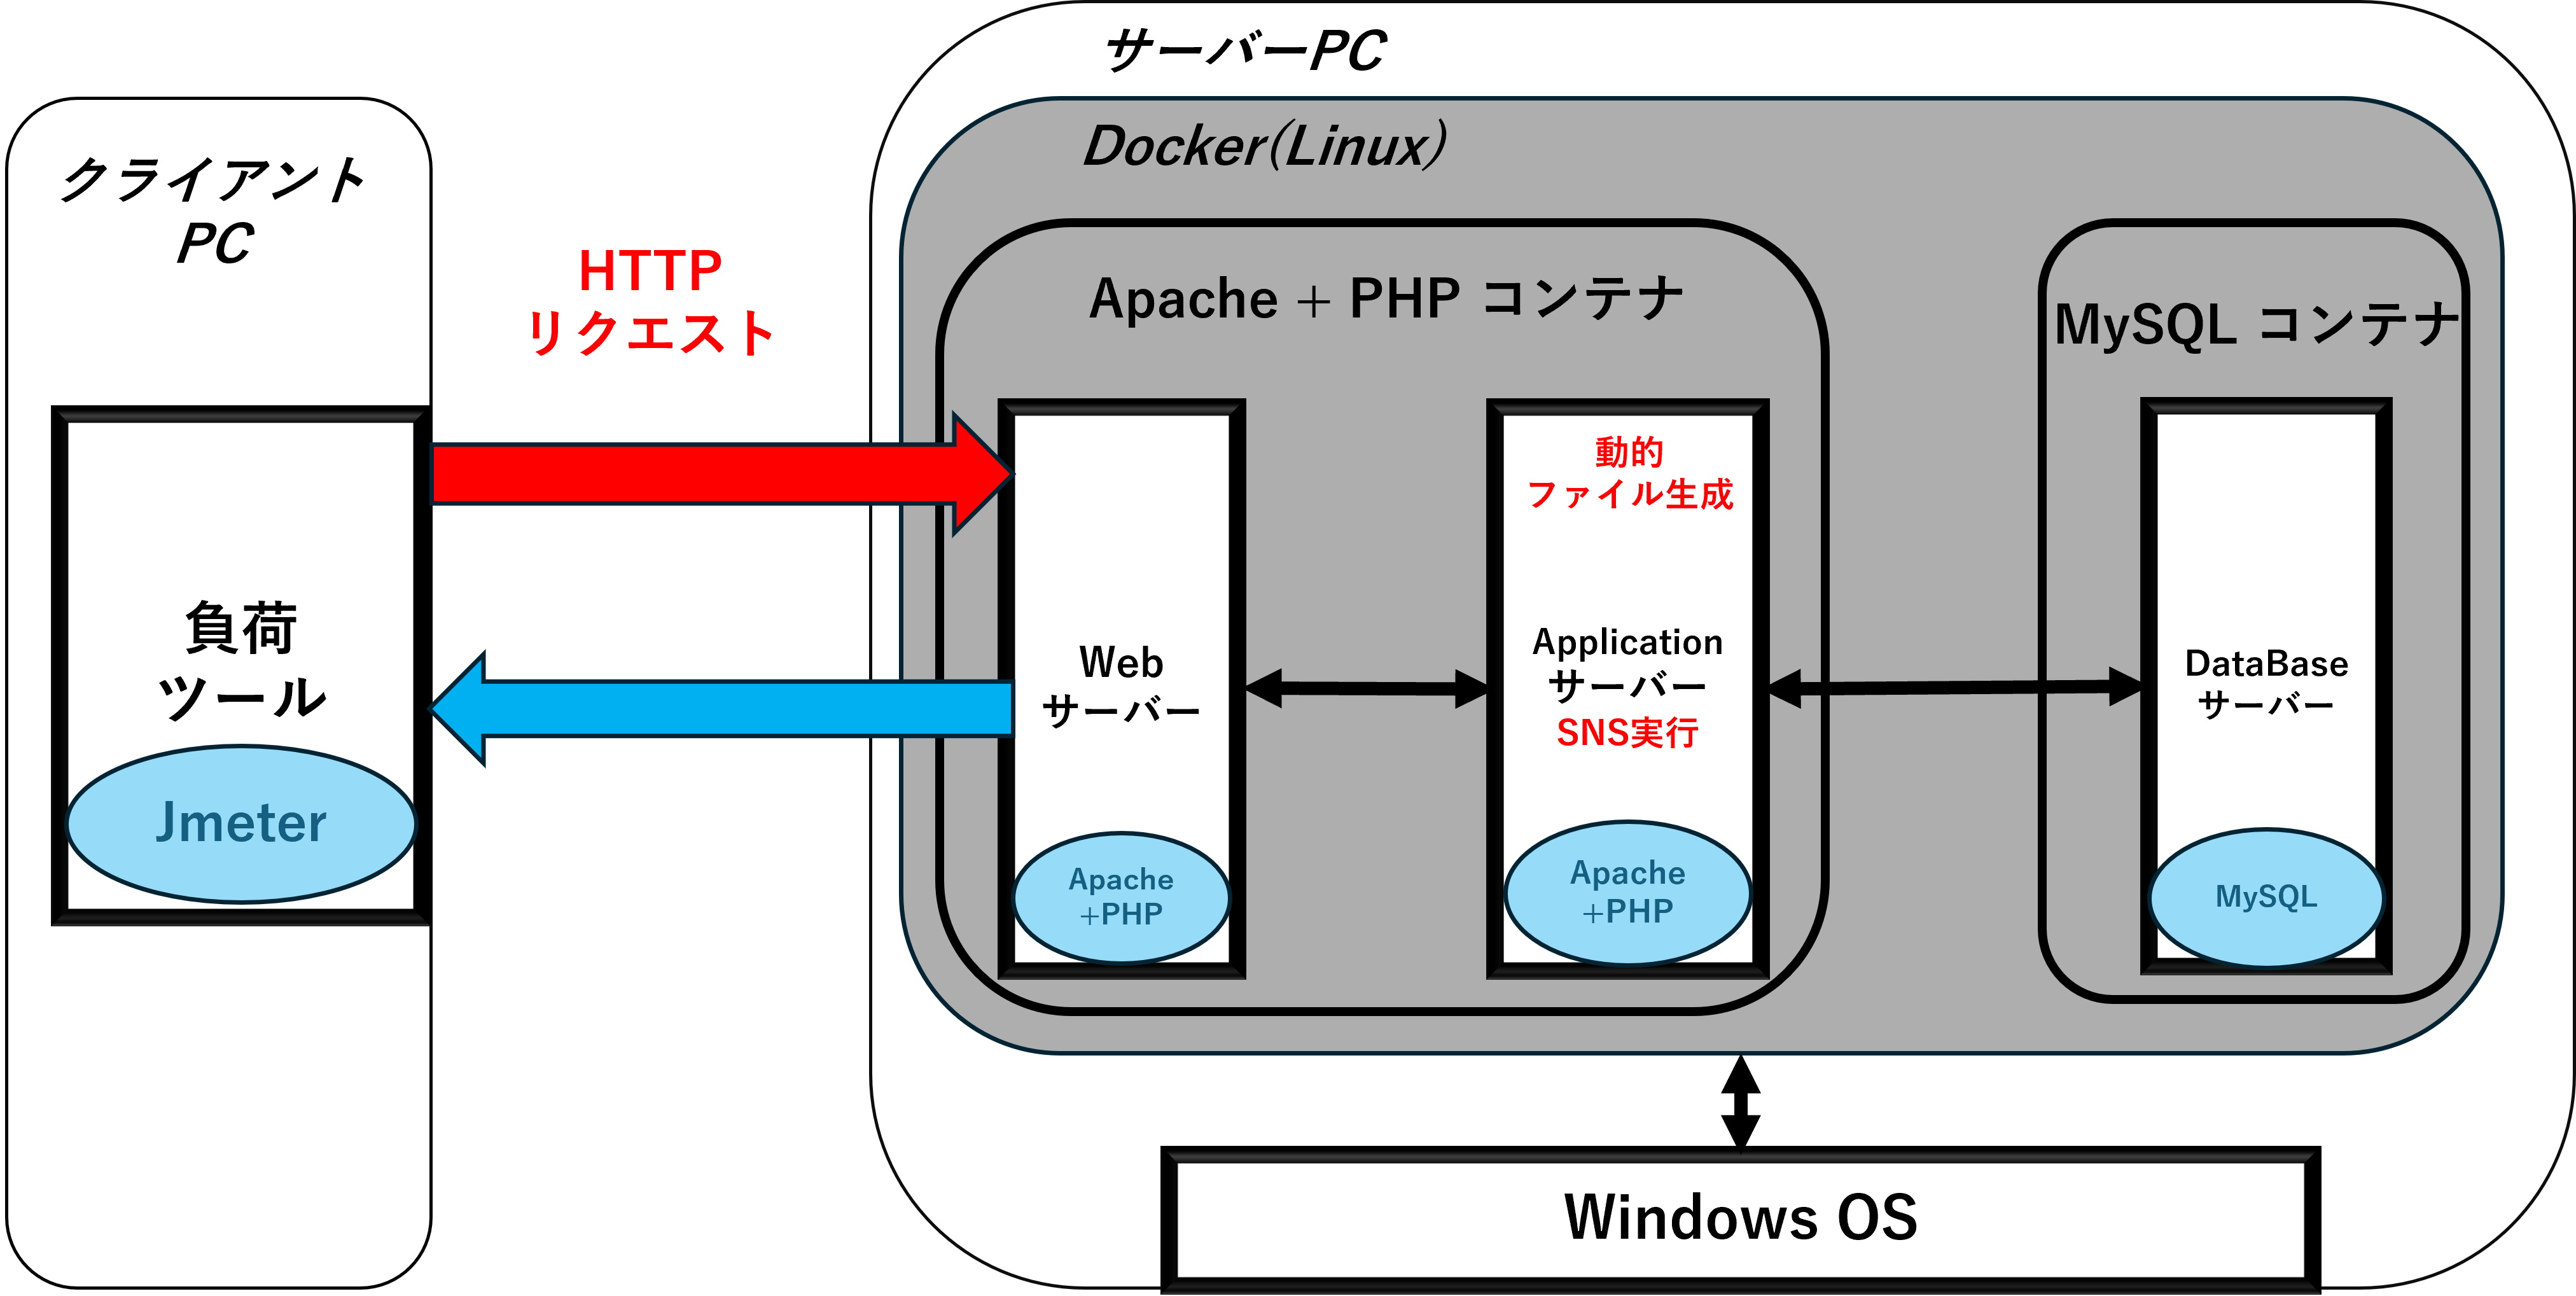
\includegraphics[scale=0.239]{figures/SNS_Docker.png}
  \vspace{-0.55cm}
  \caption{SNS運用環境と負荷ツール}
  \label{fig:1}
  \vspace{-0.15cm}
\end{figure}

\begin{table}[t]
  \vspace{-0.3cm}
  \centering
  \caption{エラー率とサーバーの性能限界}
  \label{tab:rps}
  \begin{tabular}{ccccc}
    \hline \hline
    負荷 [RPS] & 5 & 10 & 15 & 20 \\ \hline %以下差し替え
    エラー率 [\%] & 0.36 & 3.08 & 28.51 & 43.26 \\ \hline
    性能限界 [RPS] & 4.98 & 9.69 & 10.72 & 11.35 \\ \hline
  \end{tabular}
  \vspace{-0.4cm}
\end{table}

\section{実験}
本実験では,0hから1hの間に10,000スレッドを立ち上げ,その後1hから25hを負荷期間として設定する.
さらに,Torquatoら\cite{Torquato2018SWAREa}を参考に,25hから27hを監視期間として設定し,10RPSの負荷を与え,メトリクスを監視する.
なお,RPS (Requests Per Second)は負荷の大きさを表す単位である.

\subsection{本実験環境の性能調査}
\label{subsec:limit}
% 本実験環境における
本節では,負荷を5RPS,10RPS,15RPS,20RPSで与え,用意したサーバーの性能限界を推測する.

表\ref{tab:rps}にエラー率とそれに基づいて推測されたサーバーの性能限界を示す.
性能限界は,1秒間に正しく処理できるリクエスト数とし,$性能限界=負荷\times(100\%-エラー率)$により計算する.
表\ref{tab:rps}から,本実験環境の性能限界は9RPSから11RPS程度であると推測する.
なお,本節の実験では監視期間を設定していない.

\subsection{シナリオ1:一定負荷(監視期間2h)}\label{subsec:load1}

本節では現実の定常的な状況を想定した一定負荷のシナリオを考える.
\ref{subsec:limit}節の結果を踏まえ,負荷を5RPS,10RPS,15RPSと設定して,3種類のメトリクスデータを得た.
% 現実において,定常的な状況と対応する.
% 三つの負荷シナリオについて,1h~25hの負荷期間における全メトリクスは,Mann-Kendall検定\cite{Mann1945Nonparametric}により帰無仮説が否定された.
% また,Senの傾き推定\cite{Sen1968Estimates}により傾き$E$の推定値は,0.00005~0.0035の範囲と非常に小さいものの,正の値を示し,ソフトウェアエージングのリスクが発見された.
% ただし,検定の対象からは,スレッド立ち上げの影響が残る負荷期間の最初の15分を除く.
スレッド立ち上げの影響が残る負荷期間の最初の15分を除いたデータに対して,Mann-Kendall検定\cite{Mann1945Nonparametric}とSenの傾き推定\cite{Sen1968Estimates}を行った結果,前者は帰無仮説が棄却され,後者は傾きの推定値が正であることから,OpenPNEのサーバーにソフトウェアエージングのリスクが確認された.

\subsection{シナリオ2:増加負荷(監視期間2h)}\label{subsec:load2}

本節では,\ref{subsec:limit}節より推測した性能限界に近い範囲で負荷を段階的に増加させ,現実における注目度が高まる状況を想定する.
具体的には,1hから25hの間に,1RPSから15RPSまで線形に負荷を増加させる.

図\ref{f1},図\ref{f2},図\ref{f3}は,3種類のメトリクスの時系列変化を示している.
スレッド立ち上げ期間中は負荷の大きさにより,各メトリクスが比較的高い値を示している.
増加負荷の期間では,負荷の増加に伴い,全メトリクスが増加していることが確認できる.
特にエラー率は,負荷が約10RPS程度に達する16時間ごろから急激に増加しており,推測された性能限界の妥当性が確認された.
また,CPU使用率とメモリ使用量については,同時間帯までは増加傾向にあったが,それ以降は急激な増加は見られなかった.
\ref{subsec:limit}節と\ref{subsec:load1}節の結果と合わせて考えると,メモリ使用量がCPU使用率よりも先に限界に達したことが,エラー率上昇の原因と考察する.
これは,サーバー運用において予算が限られている場合,高性能なCPUを用意するよりも,メモリ容量を増やす方が効果的であることを示唆する.\par
さらに,\ref{subsec:load1}節と同様に,Mann-Kendall検定\cite{Mann1945Nonparametric}とSenの傾き推定\cite{Sen1968Estimates}を行った結果,増加負荷シナリオにおいても,OpenPNEのサーバーにソフトウェアエージングのリスクが確認された.
% ここの考察については,卒論では書く
% ことを考えると,メモリ使用の設定に問題があると考えられる.
% この主な原因は,phpのmpm\_eventモジュールが並列処理に不適な環境であることだと考えられる.
また,監視期間におけるエラー率は,直前の負荷期間のシナリオによって異なる振る舞いを見せていることが確認された.
% また,\ref{subsec:load1}節の監視期間のデータと比較すると,とCPU使用率メモリ使用量は,負荷期間の差異による監視期間のメトリクスの変動への影響は見られなかった.
% 一方で,エラー率は,負荷の程度によって,増減の範囲が大きくなるという意味で不安定になる可能性があると確認できた.
\section{結論と今後の展望}
本研究では,比較的シンプルなSNS設定を用いて,サーバーの性能限界を推測し,比較的低い一定負荷でもソフトウェアエージングのリスクが存在することを確認した.
また,監視期間のエラー率の振る舞いが負荷期間のシナリオによって異なる現象は確認されたものの,同期間のCPU使用率やメモリ使用量の振舞に同様の傾向は見られなかったことから,追加のメトリクスの観察が必要であると考えられる.
加えて,本実験では意図しないメモリ使用量の制限が確認された.
% 具体的には,コンテナに割り当てたメモリは16GB,CPUは8コアであるが,前者は25\%以下,後者は20\%~80\%程度の使用率であるにも関わらず,エラーを生じている.\par
具体的には,DockerでApache$~+~$PHPコンテナに割り当てたメモリは16GBであるが,実際のメモリ使用量は4GB(25\%)以下で停滞している.
この現象の原因究明及び,ソフトウェアエージングとの関連性の解明が課題として挙げられる.\par
\begin{figure}[t]
  \centering
  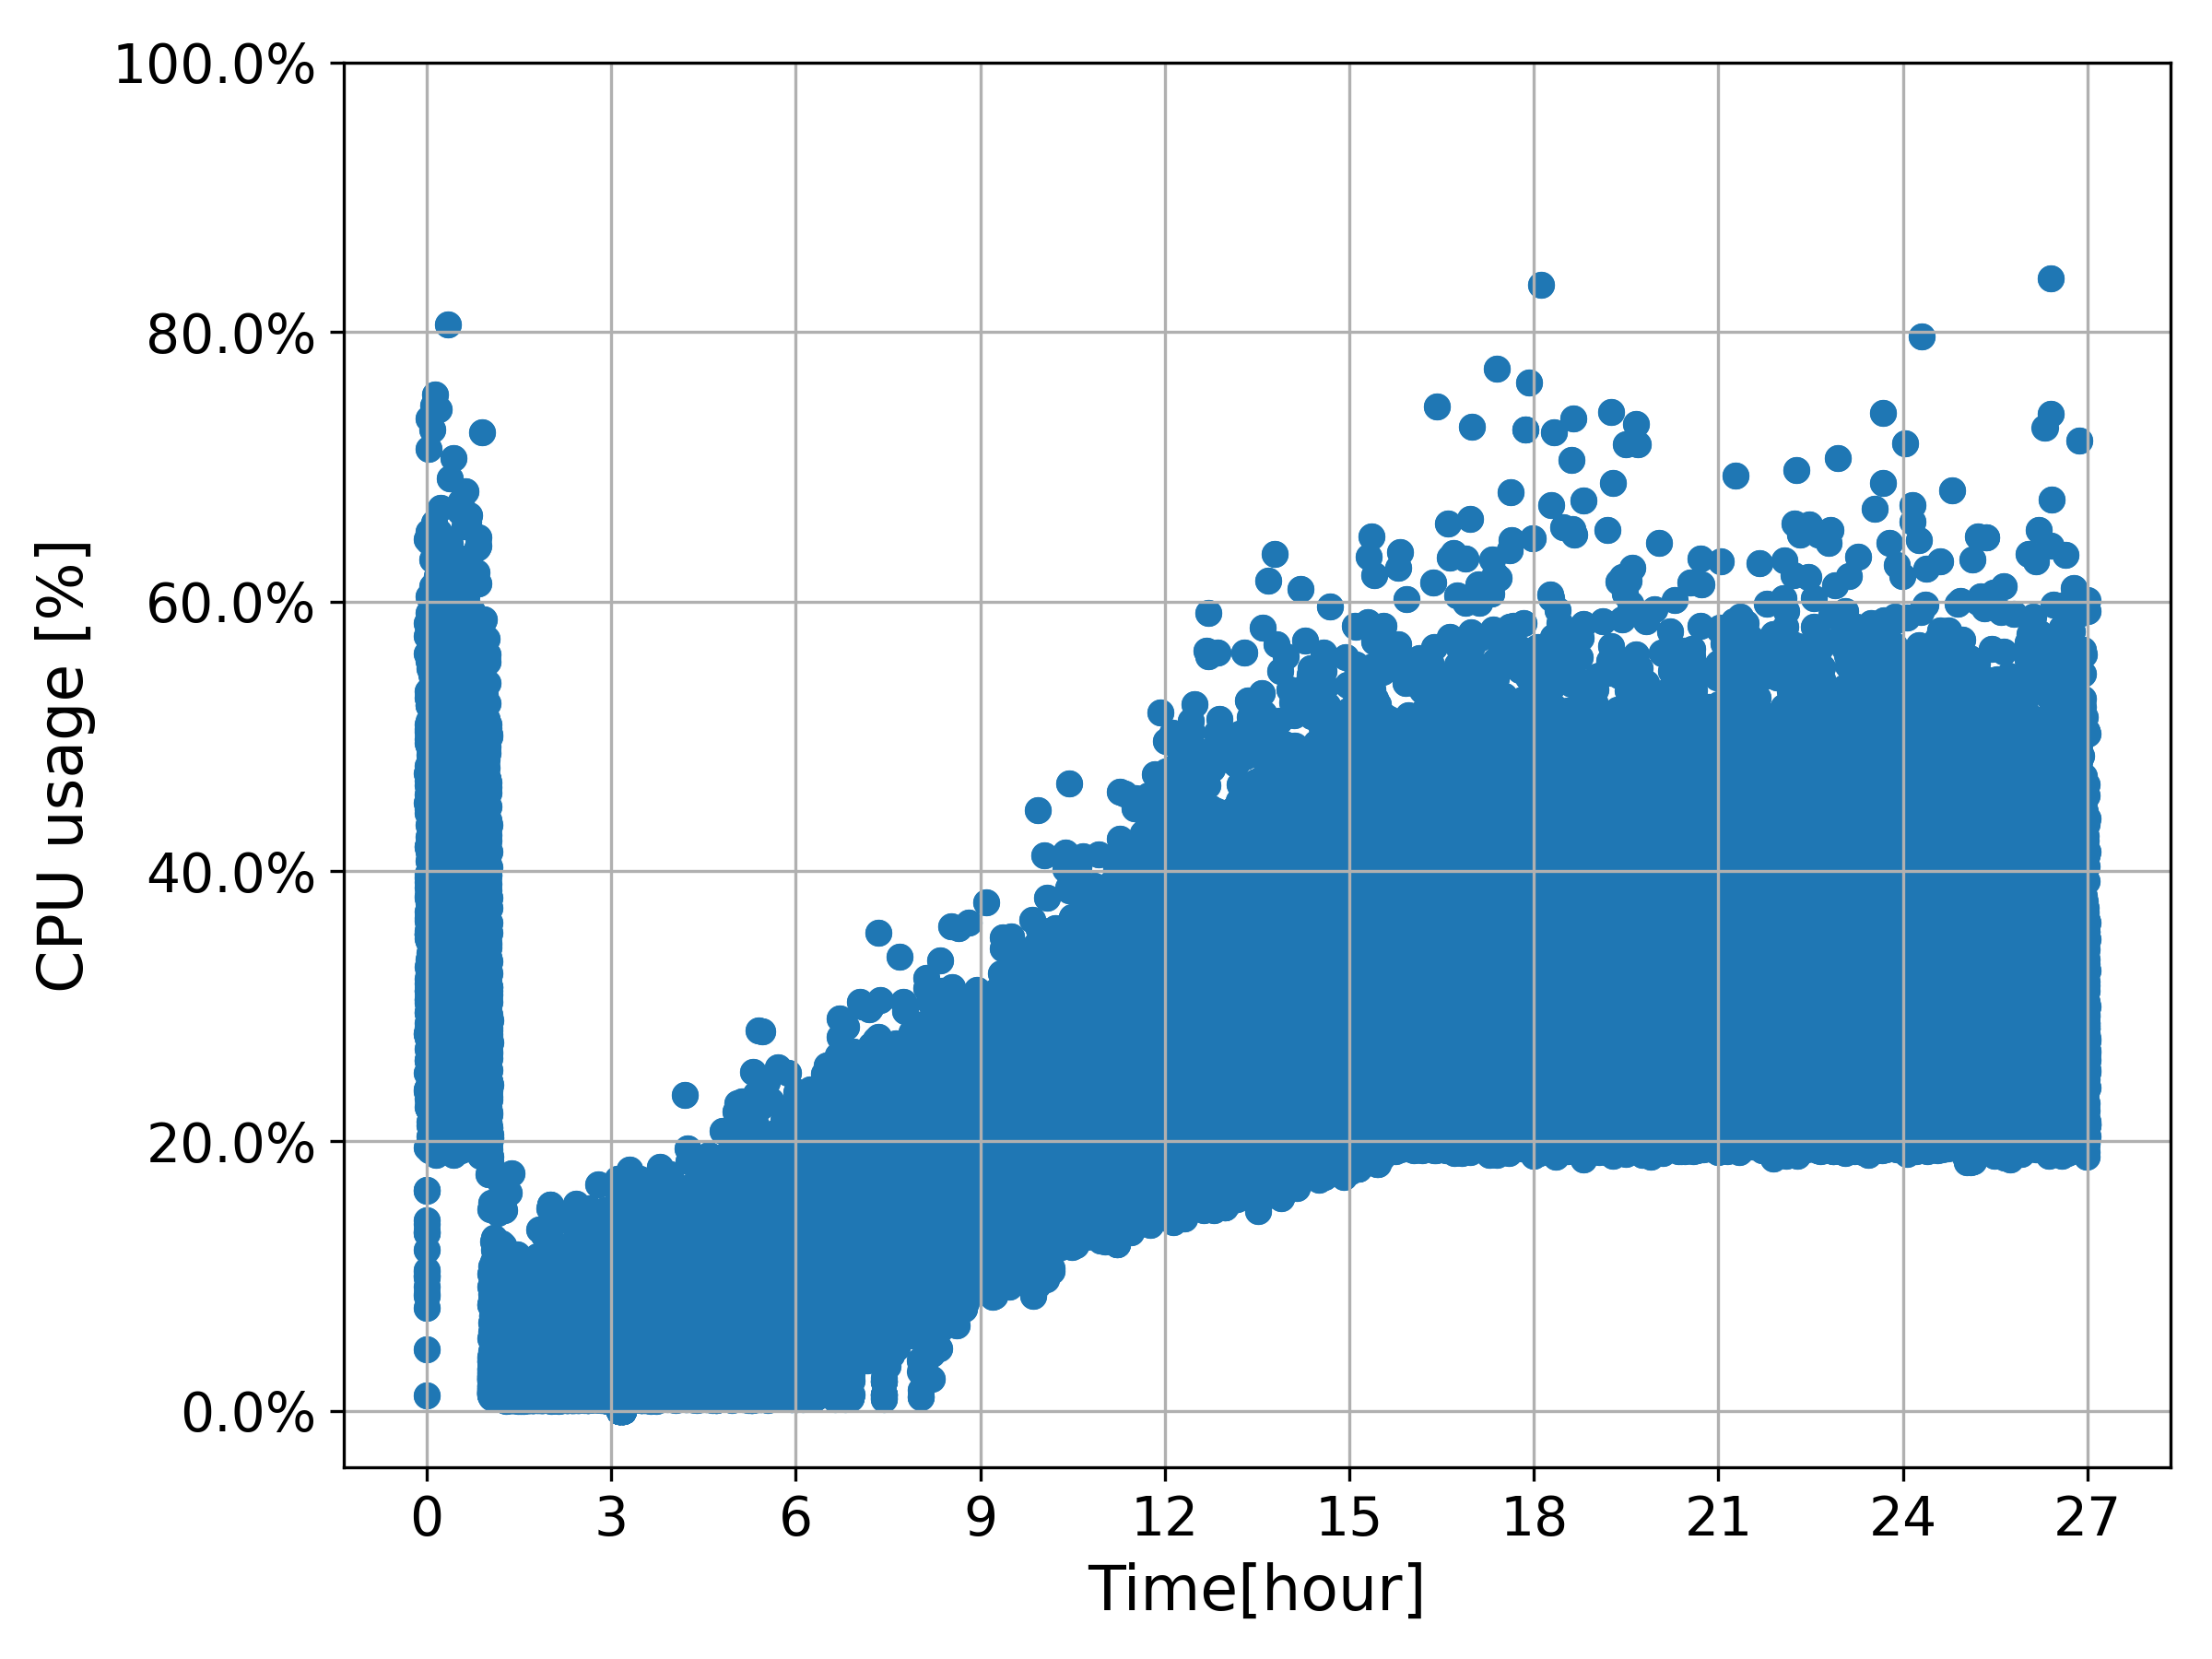
\includegraphics[width=5.2cm]{figures/8core_1_15rps_increase_cpu.png}
  \vspace{-0.5cm}
  \caption{CPU使用率}
  \label{f1}

  \centering
  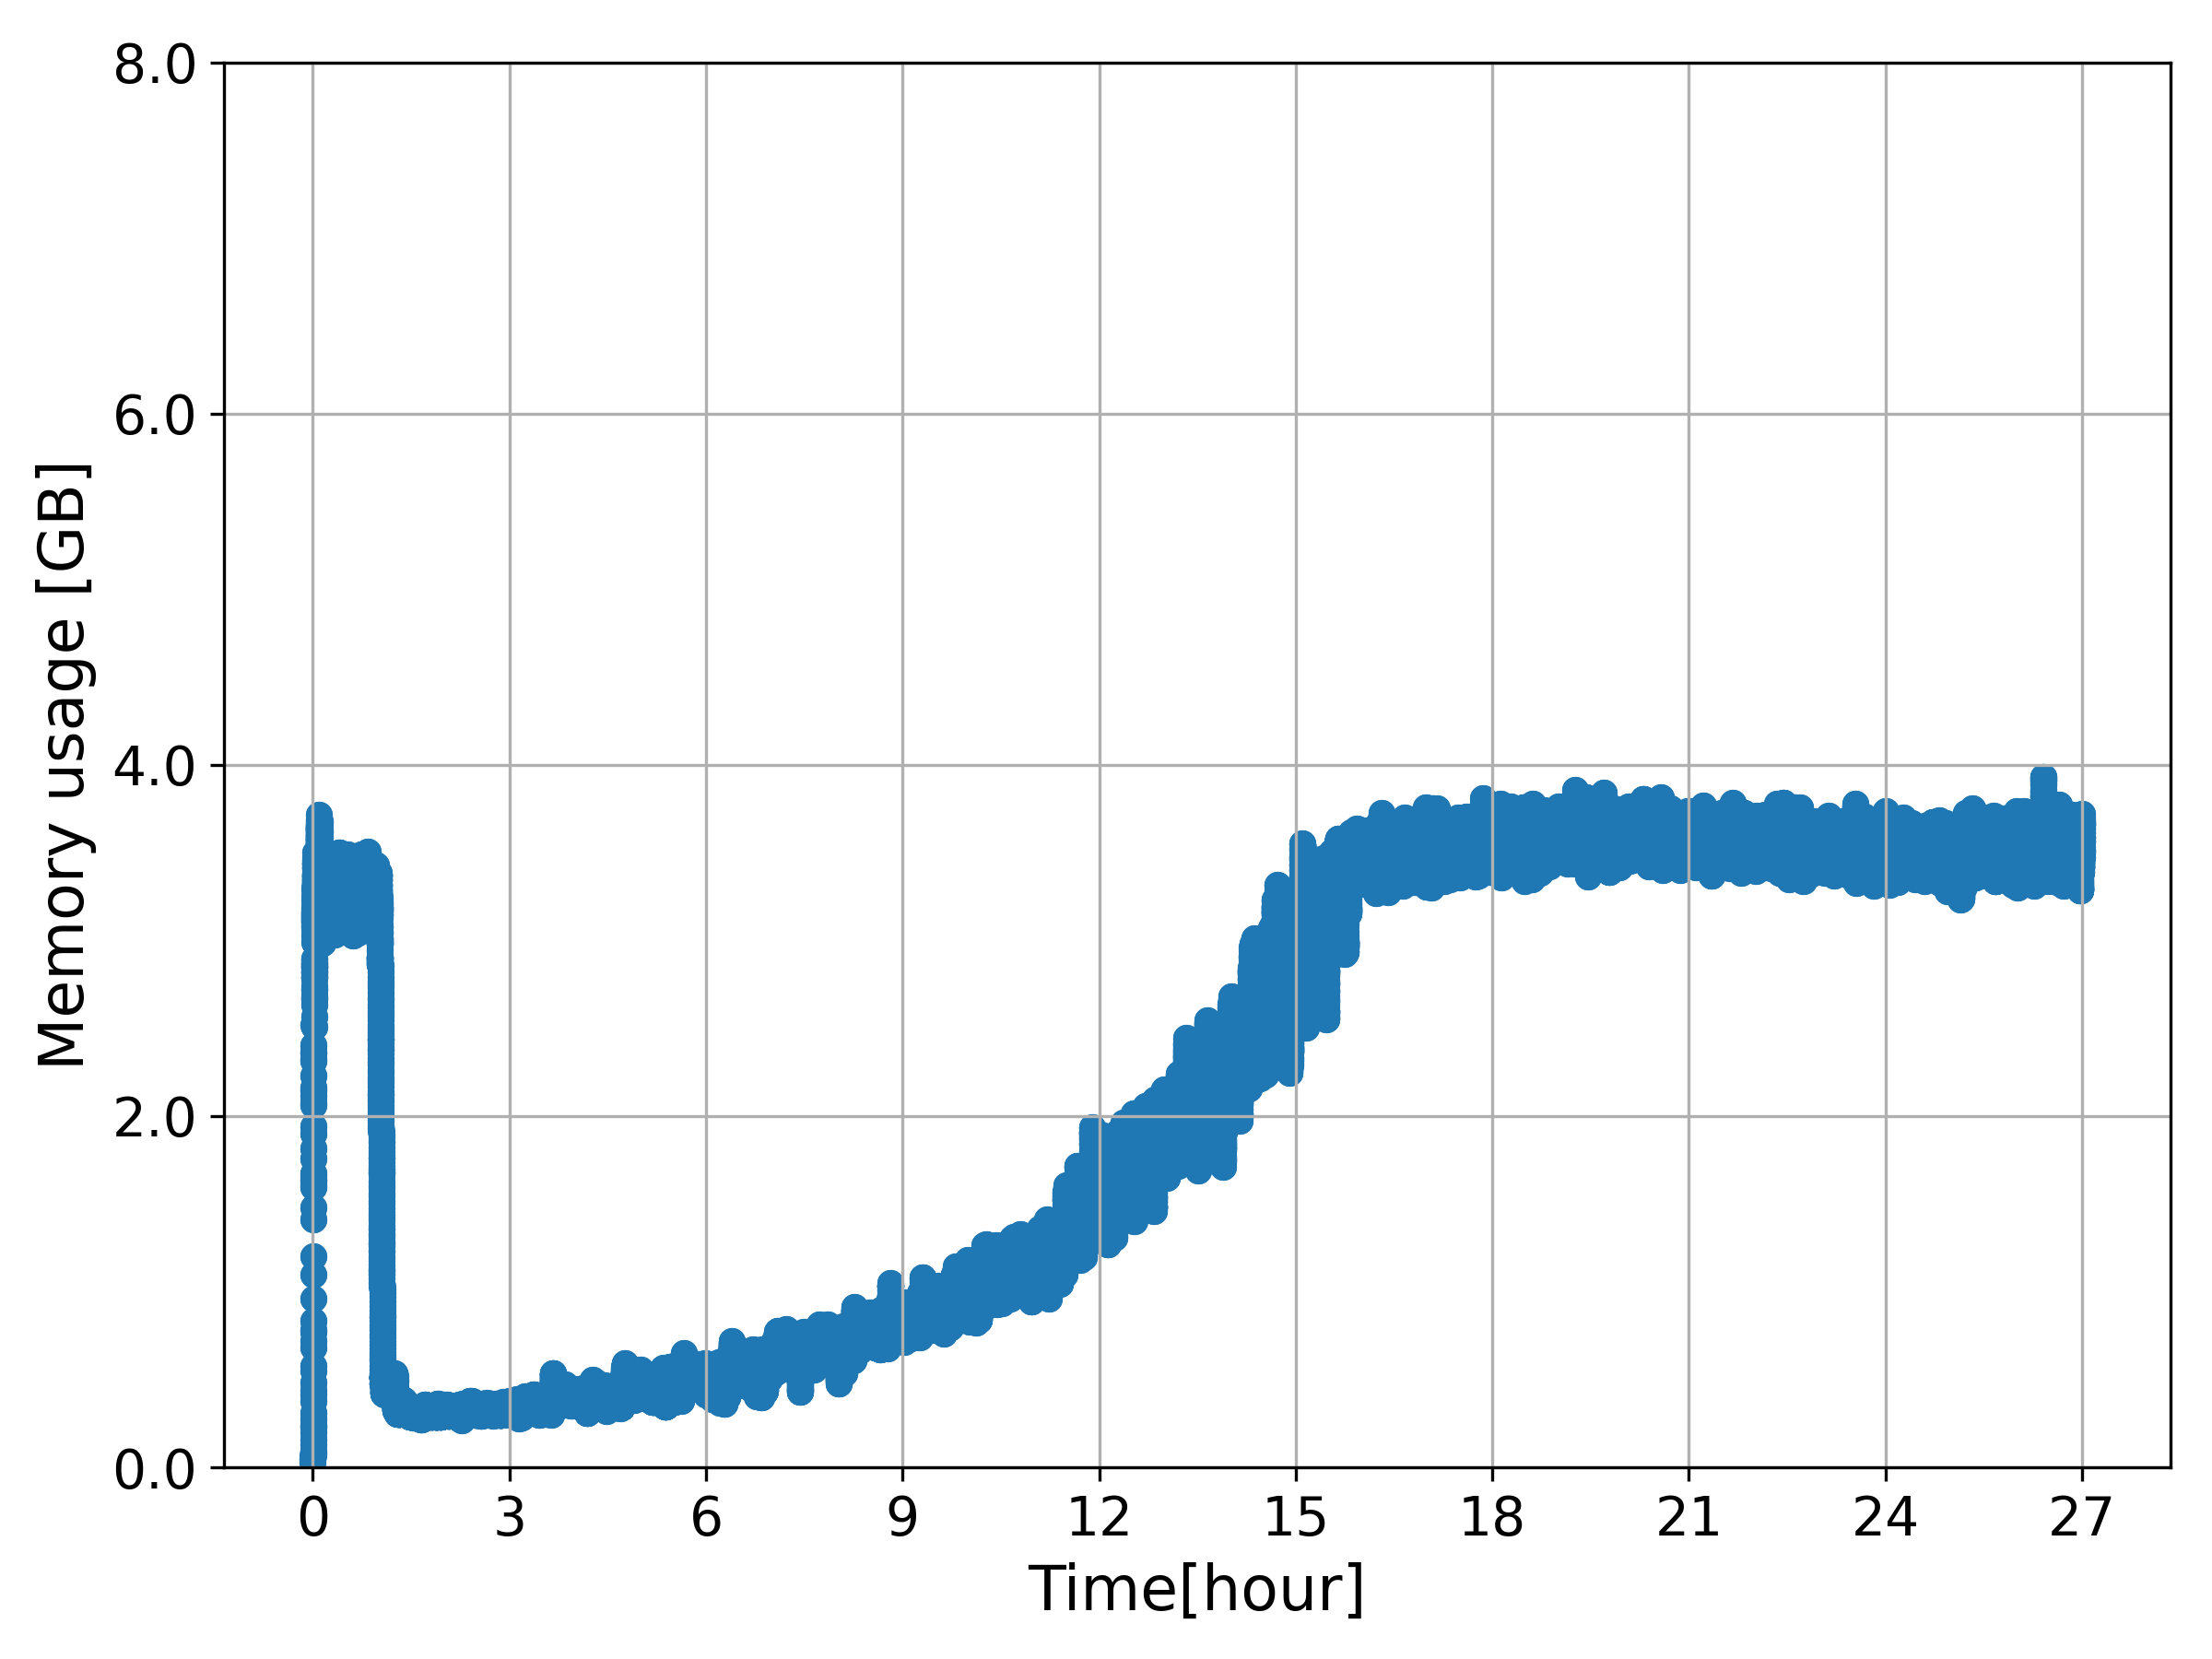
\includegraphics[width=5.2cm]{figures/8core_1_15rps_increase_mem.png}
  \vspace{-0.5cm}
  \caption{メモリ使用量}
  \label{f2}

  \centering
  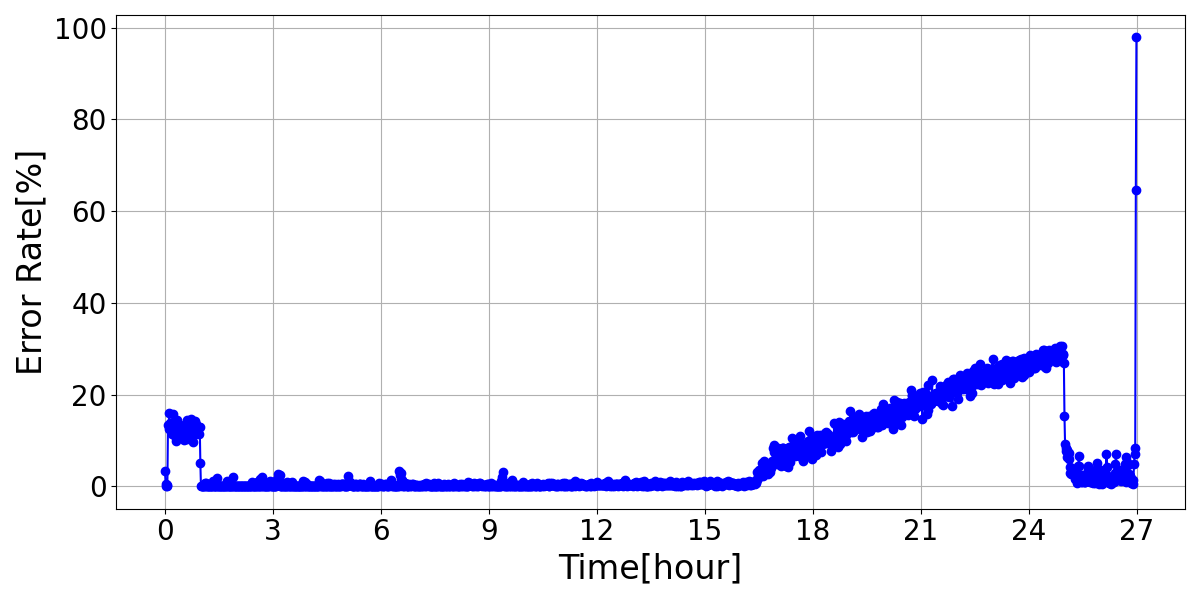
\includegraphics[width=5.4cm]{figures/or_8core_1_15_error_rate.png}
  \vspace{-0.5cm}
  \caption{エラー率}
  \label{f3}
  \vspace{-0.5cm}
\end{figure}

今後は,より高度な拡張機能を追加し,適切な設定を整えた上で,ここで得られた知見の検証を行うことが課題である.
また,近年では,SNSだけでなく,多くのWebサーバーはクラウド環境で運用されている.
従って,今後はOpenPNEをクラウド環境にデプロイし,より現実的な負荷テストを実施することが望まれる.
% $RPS=5$,RPS$=$5,RPS$~=5$
% また,本研究ではソフトウェア若化手法についての検討を行っていない.
% 再起動やガベージコレクションの管理などの代表的な若化手法を,いつ実行すべきかを検討する必要がある.


%%%%%%%%% ここから参考文献 %%%%%%%%%%%%%%%%%%%%%%%
\begin{thebibliography}{5}
  \setlength\itemsep{0.1zh}%←ここの数値を調整(行間のつまり具合)
  \setlength\baselineskip{0pt}
  \textwidth 5pt
  \vskip\baselineskip
  \setlength\baselineskip{2pt}%←ここの数値を調整(追加)(文字の大きさ)
  % \bibitem{Adams1984Optimizing}
  % Adams, N.Edward, “Optimizing Preventive Service of Software Products,” IBM Journal of Research and Development, vol. 28, no. 1, pp. 2-14, 1984.

  % \bibitem{Parnas1994Software}
  % D.L.Parnas, “Proceedings of the 16th International Conference on Software Engineering (ICSE1994),” Software aging, pp. 279-287, 1994.

  % \bibitem{Huang1995Software}
  % Y.Huang, C.Kintala, N.Kolettis and N.D.Fulton, “Software Rejuvenation: Analysis, Module and Applications,” 25th International Symposium on Fault-Tolerant Computing(FTCS1995), pp. 381-390, 1995.

  \bibitem{Dohi2020Handbook}
  T. Dohi, K. Trivedi, and A. Avritzer, \emph{Handbook of Software Aging and Rejuvenation}, New Jersey, USA: WORLD SCIENTIFIC, pp. 73--90, 2020.

  \bibitem{Torquato2018SWAREa}
  M. Torquato, J. Araujo, I. M. Umesh, and P. R. M. Maciel, “SWARE: A methodology for software aging and rejuvenation experiments,” \emph{Journal of Information Systems Engineering \& Management}, vol. 3, pp. 15, 2018.

  \bibitem{Mann1945Nonparametric}
  H. B. Mann, “Nonparametric tests against trend,” \emph{Econometrica}, vol. 13, no. 3, pp. 245--259, 1945.

  \bibitem{Sen1968Estimates}
  P. K. Sen, “Estimates of the regression coefficient based on Kendall's tau,” \emph{Journal of the American Statistical Association}, vol. 63, no. 324, pp. 1379--1389, 1968.

\end{thebibliography}
%%%%%%%%%%%%%%%%%%%%%%%%%%%%%%%%%%%%%%%%%%%%%%%%%%
\end{document}